%%%%%%%%%%%%%%%%%%%%%%%%%%%%%%%%%%%%%%%%%
% Journal Article
% LaTeX Template
% Version 1.3 (9/9/13)
%
% This template has been downloaded from:
% http://www.LaTeXTemplates.com
%
% Original author:
% Frits Wenneker (http://www.howtotex.com)
%
% License:
% CC BY-NC-SA 3.0 (http://creativecommons.org/licenses/by-nc-sa/3.0/)
%
%%%%%%%%%%%%%%%%%%%%%%%%%%%%%%%%%%%%%%%%%

%----------------------------------------------------------------------------------------
%	PACKAGES AND OTHER DOCUMENT CONFIGURATIONS
%----------------------------------------------------------------------------------------

\documentclass[twoside]{article}

\usepackage{lipsum} % Package to generate dummy text throughout this template

\usepackage[sc]{mathpazo} % Use the Palatino font
\usepackage[T1]{fontenc} % Use 8-bit encoding that has 256 glyphs
\linespread{1.05} % Line spacing - Palatino needs more space between lines
\usepackage{microtype} % Slightly tweak font spacing for aesthetics

\usepackage[hmarginratio=1:1,top=32mm,columnsep=20pt]{geometry} % Document margins
\usepackage{multicol} % Used for the two-column layout of the document
\usepackage[hang, small,labelfont=bf,up,textfont=it,up]{caption} % Custom captions under/above floats in tables or figures
\usepackage{booktabs} % Horizontal rules in tables
\usepackage{float} % Required for tables and figures in the multi-column environment - they need to be placed in specific locations with the [H] (e.g. \begin{table}[H])
%\usepackage{hyperref} % For hyperlinks in the PDF

\usepackage{lettrine} % The lettrine is the first enlarged letter at the beginning of the text
\usepackage{paralist} % Used for the compactitem environment which makes bullet points with less space between them

\usepackage{abstract} % Allows abstract customization
\renewcommand{\abstractnamefont}{\normalfont\bfseries} % Set the "Abstract" text to bold
\renewcommand{\abstracttextfont}{\normalfont\small\itshape} % Set the abstract itself to small italic text

\usepackage{titlesec} % Allows customization of titles
%\renewcommand\thesection{\Roman{section}} % Roman numerals for the sections
%\renewcommand\thesubsection{\Roman{subsection}} % Roman numerals for subsections
\titleformat{\section}[block]{\large\scshape\centering}{\thesection.}{1em}{} % Change the look of the section titles
\titleformat{\subsection}[block]{\large}{\thesubsection.}{1em}{} % Change the look of the section titles

\usepackage{fancyhdr} % Headers and footers
\pagestyle{fancy} % All pages have headers and footers
\fancyhead{} % Blank out the default header
\fancyfoot{} % Blank out the default footer
\fancyhead[C]{Autonomous Systems Engineering} % Custom header text
\fancyfoot[RO,LE]{\thepage} % Custom footer text

\usepackage{graphicx}
\usepackage{multicol}
\usepackage{tikz}
\usepackage{textcomp}
\usepackage{wrapfig}
\usepackage{floatflt}
\usetikzlibrary{shapes}
% Quellcode
\usepackage{listings}
\lstloadlanguages{C++,Python}
\definecolor{mygreen}{rgb}{0,0.6,0}
\definecolor{myblue}{rgb}{0,0,0.8}
\lstset{ %
	breaklines=true,
	basicstyle=\fontsize{10pt}{12pt}\ttfamily,
	commentstyle=\color{mygreen},
	keywordstyle=\color{myblue},
	rulecolor=\color{black},
	captionpos=b,
	language=Python,
	numbers=left,
	xleftmargin=2em,
	numberstyle=\tiny,
	framexleftmargin=1.8em,
	%numbersep=10pt,
	frame=L}
%----------------------------------------------------------------------------------------
%	TITLE SECTION
%----------------------------------------------------------------------------------------

\title{\vspace{-15mm}\fontsize{24pt}{10pt}\selectfont\textbf{Scenario and Evaluation Algorithms}} % Article title

\author{
\large
\textsc{Hendrik Oestreich, Andreas Gatting, Timo Michalski, Julian Daberkow}\\
\textsc{Julian Exner, <further Authors>}\\%\thanks{A thank you or further information}\\[2mm] % Your name
\normalsize University of Bielefeld \\ % Your institution
%\normalsize hoestreich@techfak.uni-bielefeld.com%\href{mailto:hoestreich@techfak.uni-bielefeld.com}{hoestreich@techfak.uni-bielefeld.com} % Your email address
%\vspace{-5mm}
}
\date{July 2015}

%----------------------------------------------------------------------------------------

\begin{document}

\maketitle % Insert title

\thispagestyle{fancy} % All pages have headers and footers


%----------------------------------------------------------------------------------------
%	ARTICLE CONTENTS
%----------------------------------------------------------------------------------------

%\begin{multicols}{2} % Two-column layout throughout the main article text

\section{Scenario}
\subsection{Setup} % TODO Hendrik
\subsection{Tracking Tool} % Someone else

\begin{figure} 
	\begin{centering}
		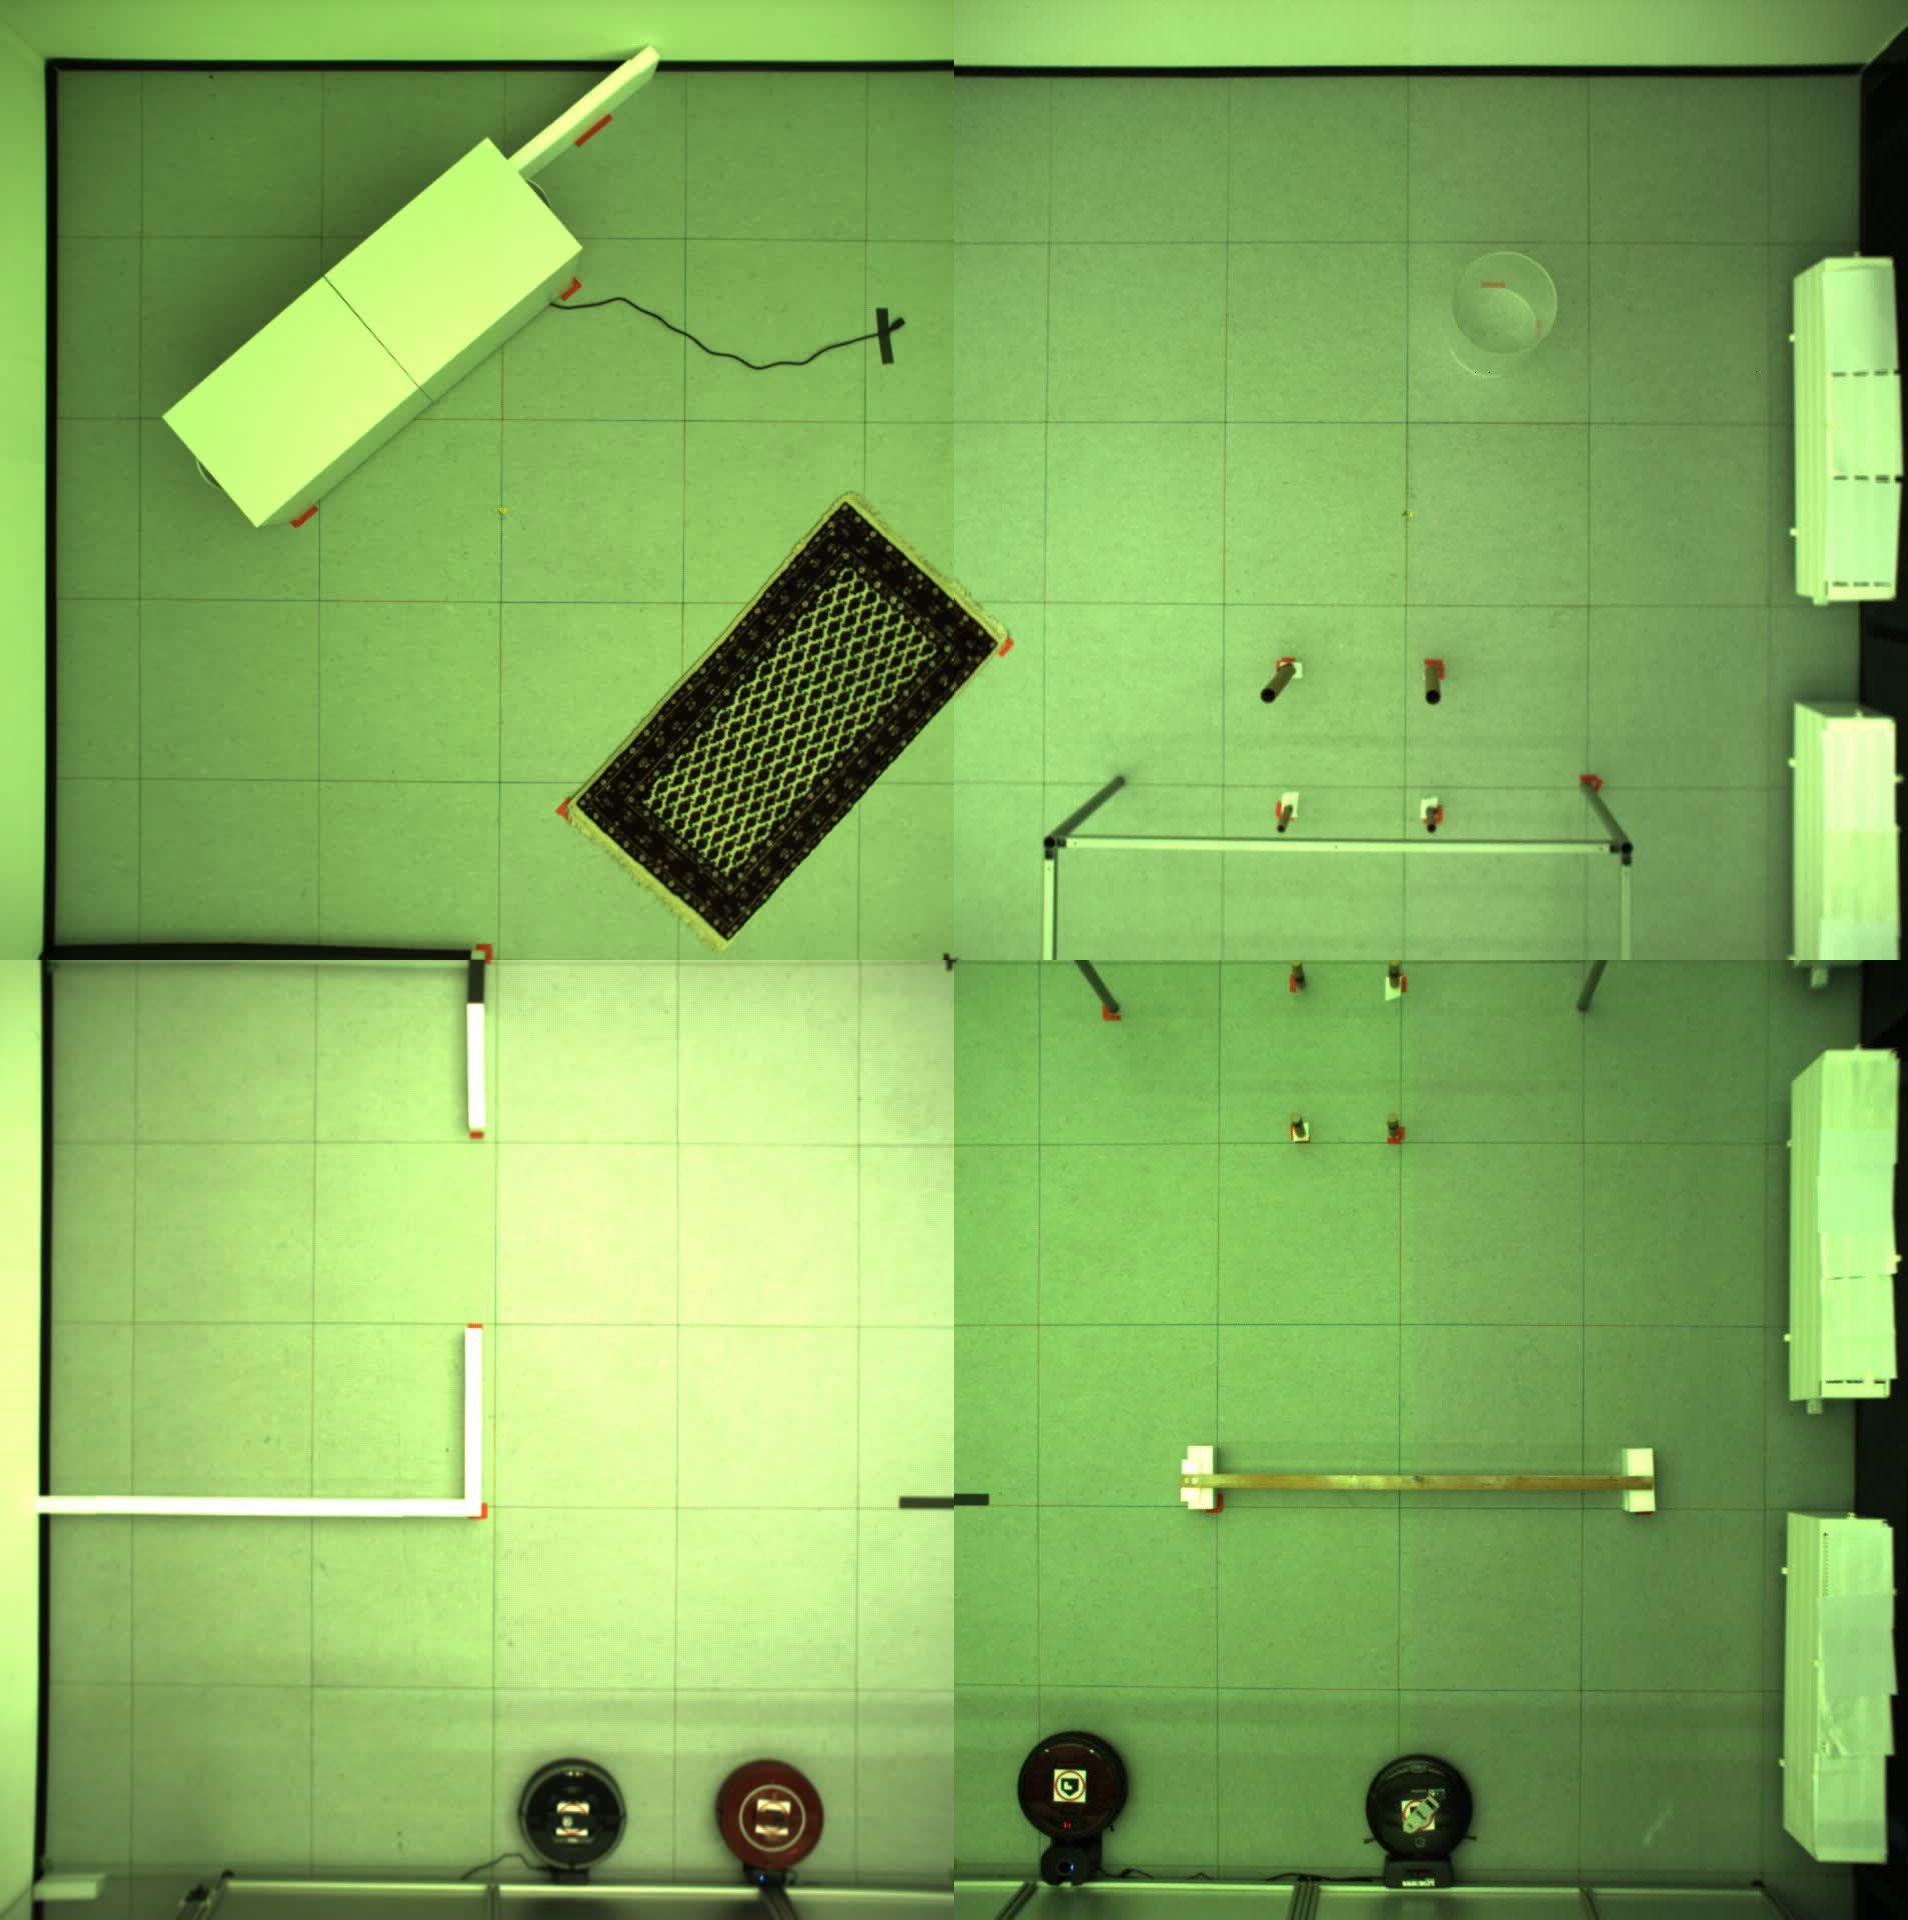
\includegraphics[width=0.5\textwidth]{setup.jpg}
		\caption{Exemplary camera picture.}
		\label{fig:setup}
	\end{centering}
\end{figure}
The tracking tool consists of four independent optical cameras, which are mounted to the ceiling and face towards the ground. Each camera provides a resolution of $1000 \times 1000$ pixel, bringing the total resolution to $2000 \times 2000$. A sample picture can be seen in Figure \ref{fig:setup}. Markers are glued to the objects that are to be tracked. Multiple objects can be tracked simultaneously. Each camera generates independent tracking data, which can be stitched with the other cameras' tracking data in the post processing step. Each entry in the tracking data contains the following elements:

\begin{itemize}
	\item Timestamp.
	\item Boolean value of either 0 or 1 depending on whether a certain marker was detected.
	\item The marker number. 
	\item X-coordinate.
	\item Y-coordinate.
	\item Turning angle.
\end{itemize}
X and Y-coordinates are given in pixel values that correspond to the marker position. 




\subsection{Execution} % TODO Andi

\section{Evalution Algorithms}
\subsection{Group 1}
\subsubsection{Preprocessing of tracking data} % TODO Hendrik
\subsection{Distance} % TODO Andi
\subsubsection{Duration} % TODO Timo
\subsubsection{Coverage} % TODO Julian D.
\subsubsection{Heatmap} % TODO Leroy

\subsection{Group 2} % TODO Julian E. & Martin
\subsubsection{Preprocessing of tracking data}
\subsubsection{Heatmap}
\subsubsection{Histogram}

%\end{multicols}

\end{document}
